\documentclass[handout]{beamer}

% Choose how your presentation looks.
%
% For more themes, color themes and font themes, see:
% http://deic.uab.es/~iblanes/beamer_gallery/index_by_theme.html
%
\mode<presentation>
{
  \usetheme{Darmstadt}      % or try Darmstadt, Madrid, Warsaw, ...
  \usecolortheme{beaver} % or try albatross, beaver, crane, ...
  \usefonttheme{serif}  % or try serif, structurebold, ...
  \setbeamertemplate{navigation symbols}{}
  \setbeamertemplate{caption}[numbered]
} 

\usepackage[english]{babel}
\usepackage[utf8x]{inputenc}
\usepackage{wrapfig}
\usepackage{graphicx}
\usepackage{wrapfig}
\title{EDACAS/MIND Lab}
\subtitle{New Student Weclome Guide}
\author{Rashmi Jha Ph.D}
\institute{University Of Cincinnati \newline 
901/915/921 Rhodes Hall \newline
Cincinnati, Ohio 45221-0030 \newline
Phone: 1 513 556 1361} 
\date{Established 2015}

\begin{document}

\begin{frame}
  \titlepage
\end{frame}

% Uncomment these lines for an automatically generated outline.
%\begin{frame}{Outline}
%  \tableofcontents
%\end{frame}

\section{Introduction}
\newcommand{\lenitem}[2][.7\linewidth]{\parbox[t]{#1}{\strut #2\strut}}
\begin{frame}{About Us}

  \mbox{}\hfill\raisebox{-\height}[0pt][0pt]{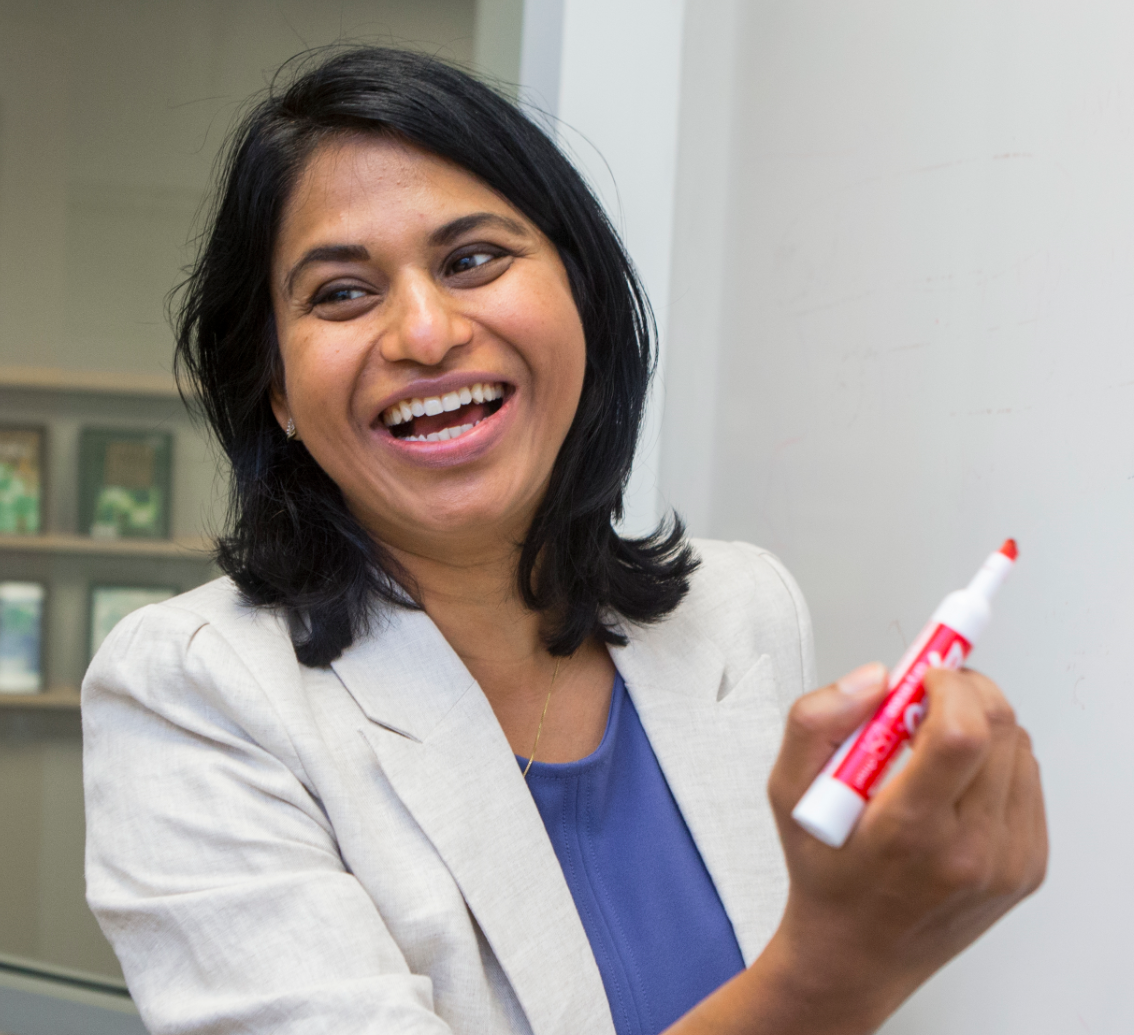
\includegraphics[width=.25\linewidth]{images/drJha.png}}
  \vspace*{-\baselineskip}

  \begin{itemize}[<+->]
  \item \lenitem{First off, welcome to the MIND Lab!}
  \item \lenitem{Say hello to Dr. Jha, she's the founder and director of the lab.}
  \item \lenitem{Dr. Jha is an Assistant Professor in the department of Electrical Engineering and Computer Systems}
  \begin{itemize}
    \item {Assistant Professor University of Toledo from 2008 to 2015.}
    \item {Process Integration Engineer at Semiconductor Research and Development Center, IBM from 2006-2008.}
    \item {Ph.D. and M.S. in Electrical Engineering from North Carolina State University in 2006 and 2003, respectively.}
  \end{itemize}
\end{itemize}
\end{frame}


\begin{frame}{Research Areas}
The lab has a wide range of research areas, including, but not limited to.....
\begin{itemize}
  \item Emerging Logic and Memory Devices beyond CMOS
  \item Neuromorphic Devices and Computing
  \item Hardware Security
  \item Cybersecurity
  \item AI in Wearables for Health
\end{itemize}
\end{frame}

\begin{frame}{So You Decided to Try Out Research}
\begin{itemize}
  \item For this guide, we'll assume that this is your first experience with any sort of research. 
  \item The first thing to remember is that research will challenge you in ways different than classroom exercises and projects have in the past
  \begin{itemize}
      \item In a way, treat this like you would treat a job in a professional setting
      \item Track your progress, set goals, document your work, etc.
  \end{itemize}
\end{itemize}
\end{frame}

\begin{frame}{Consider the Following}
\begin{itemize}
  \item The general flow of research is to find a topic, identify what hasn't been done, formulate research questions, create a testing methodology, record your results and then publish them in some academic setting (normally a conference proceedings or an academic journal).
  \begin{itemize}
      \item This is normal across all fields, and across all levels of research. 
  \end{itemize}
  \item The time it takes to complete this process will vary, depending on the research area and the project you are working on. 
  \item \begin{itemize}
      \item A good rule of thumb is to try and complete one conference level paper every year.
      \item This is more in line for a full-time graduate student, expectations are different for an Undergraduate Student or a Post-Doc.
  \end{itemize}
  \item You \textbf{will} be an expert in this field the further you get along in research. There won't be someone that can answer every question for you, although your lab mates and advisor can help you along this path
  \begin{itemize}
      \item If there already is someone who is an expert in exactly what you are doing, then your topic isn't specific enough.
  \end{itemize}
\end{itemize}
\end{frame}

\section{Where To Begin}
\begin{frame}{General Tips}
\begin{itemize}
  \item It's often recommended that you start any research based project by reading some literature in you field
  \begin{itemize}
      \item Try and find some seminal works in the area. Your advisor and fellow lab mates will have many suggestions
  \end{itemize}
  \item Google Scholar or IEEE Xplore are great tools to start your literature search
  \begin{itemize}
      \item The best source (and often the most underutilized) is the UC Engineering library. Their staff can greatly help you with your literature searches, and its always helpful to get them involved early on in your research process.
      \item More info on this can be found later in the guide
  \end{itemize}
\end{itemize}
\end{frame}

\begin{frame}{So What Should Be My Goal?}
Your individual goals should be determined by your advisor and yourself. But in general, these are the the \textit{general} steps involved with academic research
\begin{itemize}
  \item Identify a problem domain
  \begin{itemize}
      \item Pick a general field of interest (Cybersecurity, high level computing, hardware security, neuromorphic computing)
  \end{itemize}
  \item Critical discussion of what's been done
  \begin{itemize}
      \item Start to narrow down what topics you like the above field. IE. Hardware security approaches on FPGAs.
  \end{itemize}
  \item Identifications of the knowledge gaps
  \begin{itemize}
      \item What question's posed from the paper's you have read haven't been answered? What questions do you have now that you are familiar with the field?
  \end{itemize}
  \item Forming a research question
  \begin{itemize}
      \item Draft up 2-3 questions that you would like to answer with your research. 
  \end{itemize}
\end{itemize}
\end{frame}

\begin{frame}{Graduate Students}
\begin{itemize}
  \item Welcome to the rest of your life..... Just kidding great choice!
  \item Graduate School will be very different from your time as an Undergraduate.
  \begin{itemize}
      \item Your course load will be less, with often less homework. With that being said, you'll need to treat being a student as a full time job. 
      \item As a Research Assistant, you'll be expected to work for 20 hours a week on research related materials. Hours vary as a teaching assistant.
      \item There isn't someone standing over your shoulder pushing you to do research everyday, you'll have to be self-motivated.
  \end{itemize}
  \item The beginning of any research project seems very daunting, and can often be off-putting. Looks to the others around you for support and guidance!
  \item Are you excited to have summers off again? Well bottle that excitement up.
  \begin{itemize}
      \item Although you might not be taking any courses, if you are in an RA or TA position you'll still be expected to do 20 hours of research related work a week.
      \item This is a great time to get ahead of the curve towards your thesis/dissertation and work on a fall publication
  \end{itemize}
\end{itemize}
\end{frame}

\begin{frame}{Undergraduate Students}
\begin{itemize}
  \item Welcome to the lab! Undergraduate research is a great way to gauge if pursuing a career in R&D or academia is right for you!
  \item Your research expectations will be different than your fellow lab members, so make sure to discuss this with your advisor.
  \begin{itemize}
      \item Make sure you identify how many hours a week your advisor would like to work, since you will clock in and out. 
      \item Treating research like another class is a great way to balance the workload.
      \item Your lab mates will have lots of advice and experiences to share, so go to them with any questions!
  \end{itemize}
  \item This position will challenge you in different ways then your previous courses have, so be ready to change your approach to work.
\end{itemize}
\end{frame}

\begin{frame}{General Expectations}
\begin{itemize}
  \item Every week you will upload a short presentation showing what you did in the previous week, and then what you plan do to in the next week 
  \begin{itemize}
      \item We then present these in our weekly meetings, on Mondays mornings. 
      \item The presentations are also needed in case there is an audit over any of our grants, so even if you will be absent from the meeting it is important to still upload something.
  \end{itemize}
  \item You might have other meetings besides the weekly lab meeting, including some one-on-ones with your advisor or with your funding benefactors.
  \item At the end of every semester (yes, including summer) you will write a short 3 page summary in IEEE format over what you accomplished that semester. 
\end{itemize}
\end{frame}

\subsection{Tools and Resources}

\begin{frame}{Lab Equipment}
\begin{itemize}
  \item We have various pieces of equipment available for you to use in your research. The following link will take you to our equipment list and their subsequent 'owners'
  \begin{itemize}
      \item Link -> ***INSERT LINK****
  \end{itemize}
  \item We currently have three high end computers that you can use for simulations. All three have remote desktop options.
  \item \begin{itemize}
      \item Dracarys - Cyber PC (FPGA Software)
      \item Despacito - High End CPU
      \item Minesweeper Machine - High End GPU 
  \end{itemize}
\end{itemize}
\end{frame}

\begin{frame}{Reference Managers}
\begin{itemize}
  \item Start using a reference manager right away! This will save you lots of time and effort once you start working on publishing your work.
  \begin{itemize}
      \item Some popular choices are Mendeley, Zotero, RefWorks and EndNote. 
      \item Make sure to backup your database of references at least once a month! These systems aren't perfect, and sometimes encounter errors.
  \end{itemize}
  \item However you chose to read your papers (laptop, phone, printed on paper) try and highlight which portions of the paper you found useful. Some students will write a short 1-2 paragraph summary of what they learned from the paper.
  \begin{itemize}
      \item This will save you from having to re-read the full paper to remember what you need to cite from the work
  \end{itemize}
  \item Bibtex files are a great way to store your references for publications, and has an easy interlay with laTex files. 
\end{itemize}
\end{frame}

\begin{frame}{Databases}
\begin{itemize}
  \item SAVE SAVE SAVE SAVE! Its a good rule of thumb to save important files and documents in multiple places. You \textbf{will} encounter some sort computer or back-up drive failure, so get into habit of backing up your data frequently
  \begin{itemize}
      \item Popular choices are OneDrive, Google Drive, DropBox.
      \item UC gives you *unlimited* storage through OneDrive, take advantage of it!
      \item We also have a group OneDrive where we upload out weekly reports, and share resources. Ask a fellow lab member for the link.
  \end{itemize}
  \item If you are doing any sort of programming, start to use GitHub or GitLab to save your projects. 
  \begin{itemize}
      \item This can also be useful to make your datasets/programs publicly available.
      \item Commit often, perfect later. 
  \end{itemize}
\end{itemize}
\end{frame}

\begin{frame}{Other Programs}
\begin{itemize}
  \item LaTex is a great tool for academic writing. Conferences/journals will often upload their own latex formatting files for you to use, which will save you tons of time. 
  \begin{itemize}
      \item Overleaf is a good place to start, there are many examples of IEEE formatted papers and other presentations.
  \end{itemize}
  \item There are various websites that will be useful to you in academia. 
  \item Get ready to learn and love styling formats. IEEE format is the standard for our work, but other formats like APA or Chicago might be used by various publication sources.
\end{itemize}
\end{frame}

\begin{frame}{People to Know}
\begin{itemize}
  \item Adam Kunkel - System's Administrator. Adam will be your best source with any Linux Server issues, or software management.
  \item Julie Munchen - Academic Director. Julie is one of your best resources for any problem you might have. If you don't know where to go, start with her.
  \item Anthony (Tony) Seta - Grant Administrator. Tony handles most of the financial works related to your funding. 
  \item Dr. Marc Cahay - Department Head. Dr. Cahay is the head of EECS, and is good person to know.
  \item Dr. Ali Minai - Graduate Student Director. Dr. Minai is the current graduate student director, you might need his signature on a form.
  \item Teresa Hamad - Program Manager. Teresa helps manage the course offerings each semester, and helps dictate degree requirements.
  \item Dr. Wen Ben Jones - TA Manager. If you want/need to work as a Teaching Assistant, Dr. Jone is the person to talk to.
\end{itemize}
\end{frame}

\begin{frame}{Important Links}
\begin{itemize}
  \item \textbf{ALWAYS} have the most up to date version of the graduate student handbook available for reference. It will be your guide for course planning and degree requirements.
  \item Link to the MIND Lab website
  \item 
\end{itemize}
\end{frame}


% Commands to include a figure:
%\begin{figure}
%\includegraphics[width=\textwidth]{your-figure's-file-name}
%\caption{\label{fig:your-figure}Caption goes here.}
%\end{figure}

\section{References}
\begin{frame}{References}
\begin{itemize}
  \item Ref 1, probably from bibtex file
\end{itemize}
\end{frame}

\begin{frame}{Change Log}
\begin{itemize}
  \item Document created: 8-13-20 BK
\end{itemize}
\end{frame}


\end{document}
